\section{Introduction}

Prediction of the future state of complex systems is a fundamental challenge of science and engineering, and ultimately integral to the functioning of society.
Some of these systems include weather \cite{weather-violence2013}, health \cite{ginsberg2008detecting}, the economy \cite{sornette2006predictability}, marketing \cite{asur2010predicting} and transportation \cite{savely1972}.
For weather in particular, predictions are made using supercomputers integrating numerical weather models, projecting our current best guess of the weather into the future.
The accuracy of these predictions depends on the accuracy of the models themselves, and the quality of our knowledge of the current state of the atmosphere.

Model accuracy has improved with better meteorological understanding of weather processes and advances in computing technology \cite{bauer2015quiet}.
To solve the initial value problem, techniques developed over the past 50 years are now broadly known as {\em data assimilation} (DA).
Formally, data assimilation is the process of using all available information, including short-range model forecasts and physical observations, to estimate the current state of a system as accurately as possible \cite{yang2006}.
The best-guess of the current state is often referred to as the {\em analysis} state.

Here, we employ a fluid dynamics experiment as a test bed for improving numerical weather prediction algorithms, focusing specifically on data assimilation methods.
Our approach is inspired by the historical development of current methodologies, and provides a tractable system for rigorous analysis.
The experiment is a thermal convection loop, which by design simplifies our problem into the prediction of convection.
The thermosyphon, a type of natural convection loop or non-mechanical heat pump, can be likened to a toy model of climate \cite{harris2011predicting}.
The dynamics of thermal convection loops have been explored under both periodic \cite{keller1966} and chaotic \cite{welander1967,creveling1975stability,gorman1984,gorman1986,ehrhard1990dynamical,yuen1999,jiang2003,burroughs2005reduced,desrayaud2006numerical,yang2006,ridouane2010} regimes.
A full characterization of the computational behavior of a loop under flux boundary conditions by Louisos et. al. describes four regimes: chaotic convection with reversals, high Rayleigh number (Ra) aperiodic stable convection, steady stable convection, and conduction/quasi-conduction \cite{louisos2013}.
For the remainder of this work, we focus on the chaotic flow regime.

We perform all computational simulations of the thermal convection loop with the open-source finite volume C++ library OpenFOAM \cite{jasak2007}.
The open-source nature of this software enables its integration with the data assimilation framework that our present work provides.

\section{Physical Experiment and Computational Model}

\begin{figure}[t!]
  \centering
  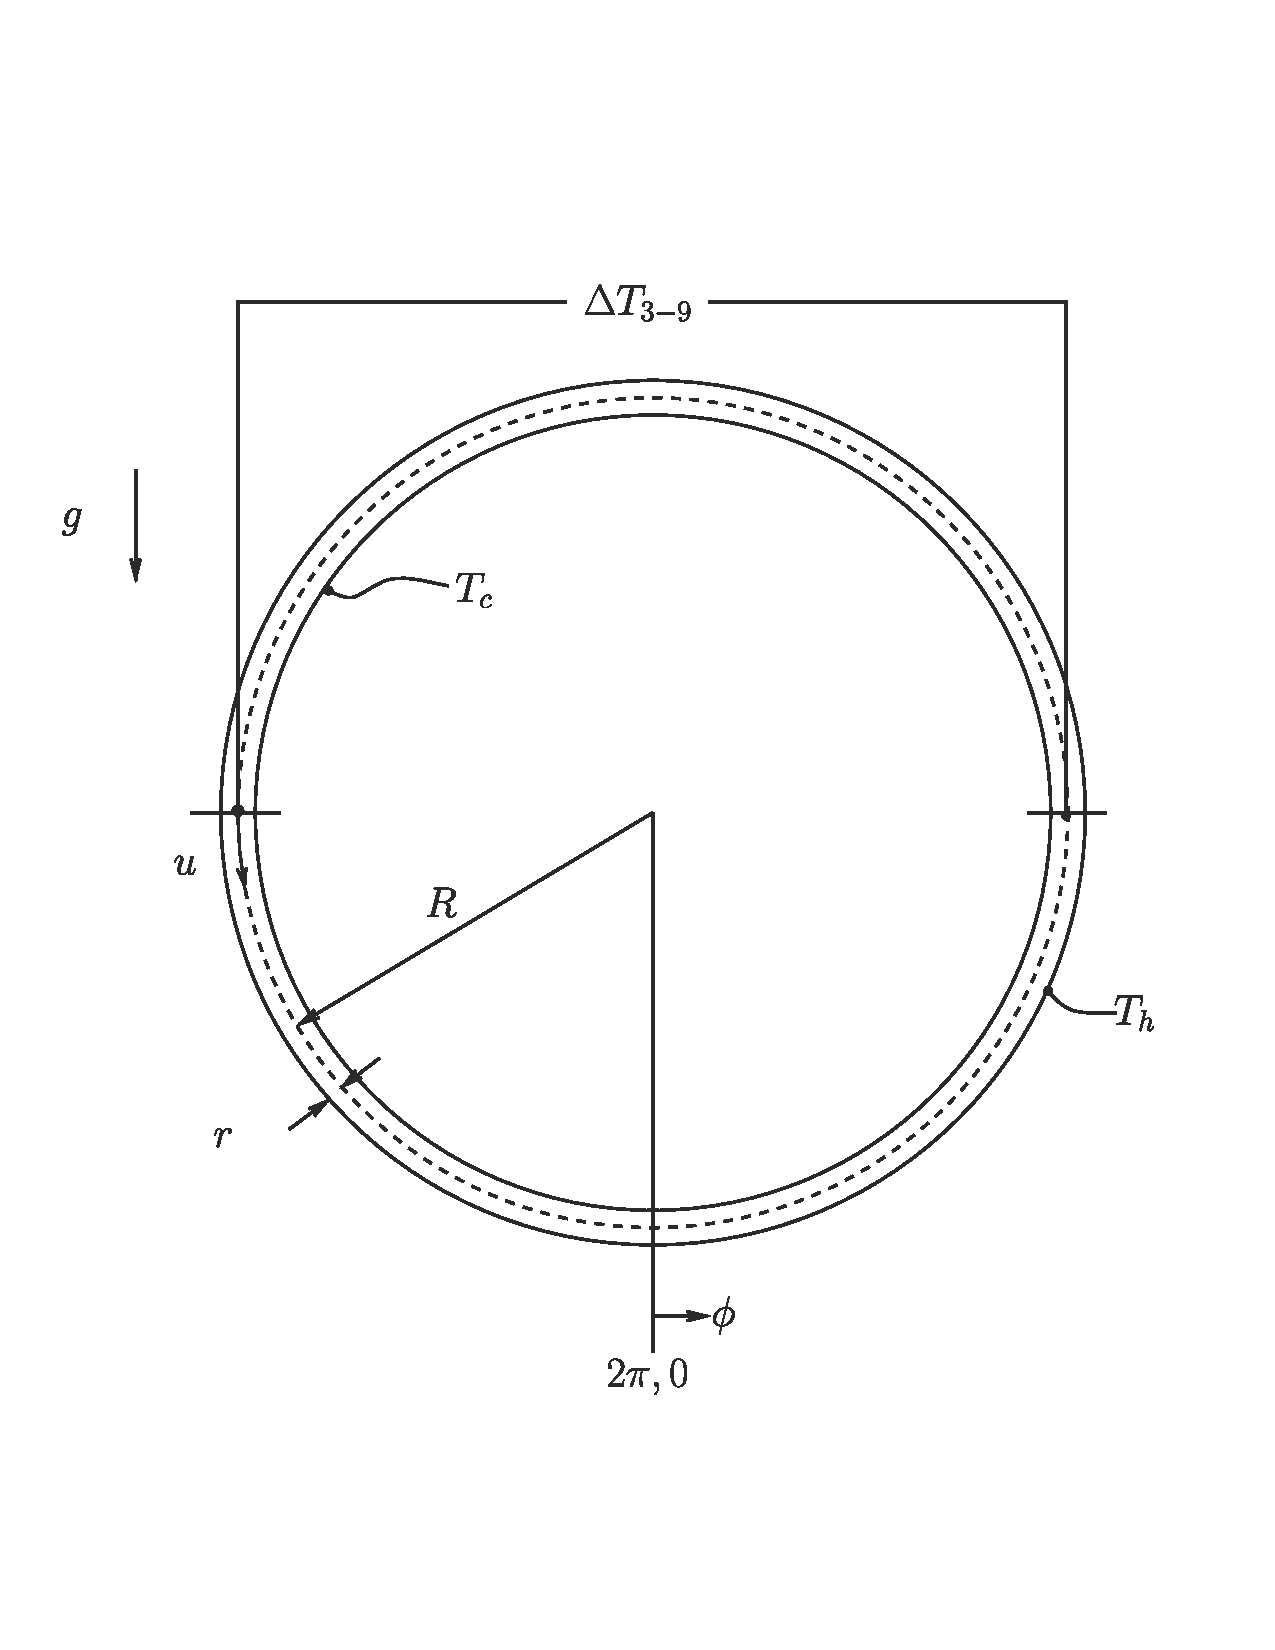
\includegraphics[width=0.45\textwidth]{figures/harris-tellus-2012-loop.pdf}
  \caption[Schematic of the experimental, and computational, setup from Harris \etal (2012)]{
    Schematic of the experimental, and computational, setup from Harris \etal (2012).
    The loop radius is given by $R$ and inner radius by $r$.
    The top temperature is labeled $T_c$ and bottom temperature $T_h$, gravity $g$ is defined downward, the angle $\phi$ is prescribed from the 6 o'clock position, and temperature difference between 3 o'clock and 9 o'clock posititions $\Delta T_{3-9}$ is labeled.
  }
  \label{fig:thermosyphon-schematic}
\end{figure}

The reduced order system describing a thermal convection loop was originally derived by Gorman \cite{gorman1986} and Ehrhard and M\"{u}ller \cite{ehrhard1990dynamical}.
Here we present this three dimensional system in non-dimensionalized form.
In Appendix B, we present a more complete derivation of these equations, following the derivation of Harris \cite{harris2011predicting}.
For the mean fluid velocity $\diff{x_1}{t}$, temperature difference between the 3 o'clock and 9 o'clock positions $\diff{x_2}{t}$ (also referred to presently as $\Delta T_{3-9}$), and deviation from conductive temperature profile $\diff{x_3}{t}$, these equations are:
\begin{align}
& \diff{x_1}{t} = \alpha (x_2 - x_1),\\
& \diff{x_2}{t} = \beta x_1 - x_2 (1 + Kh(|x_1|)) - x_1x_3,\\
  & \diff{x_3}{t} = x_1x_2 - x_3 (1 + Kh(|x_1|)) .\end{align}
The function $h(x)$ is a defined piecewise analytic polynomial, and is provided in the full derivation as Equation \ref{eq:h_defined}.
The parameters $\alpha$, $\beta$, and $K$, along with scaling factors for time and each model variable can be fit to data using standard parameter estimation techniques.

%% generated figure by /Users/andyreagan/work/2013/05-data-assimilation/thermosyphon/timeseries-plot.ipynb
\begin{figure}[h!]
  \centering
  %% 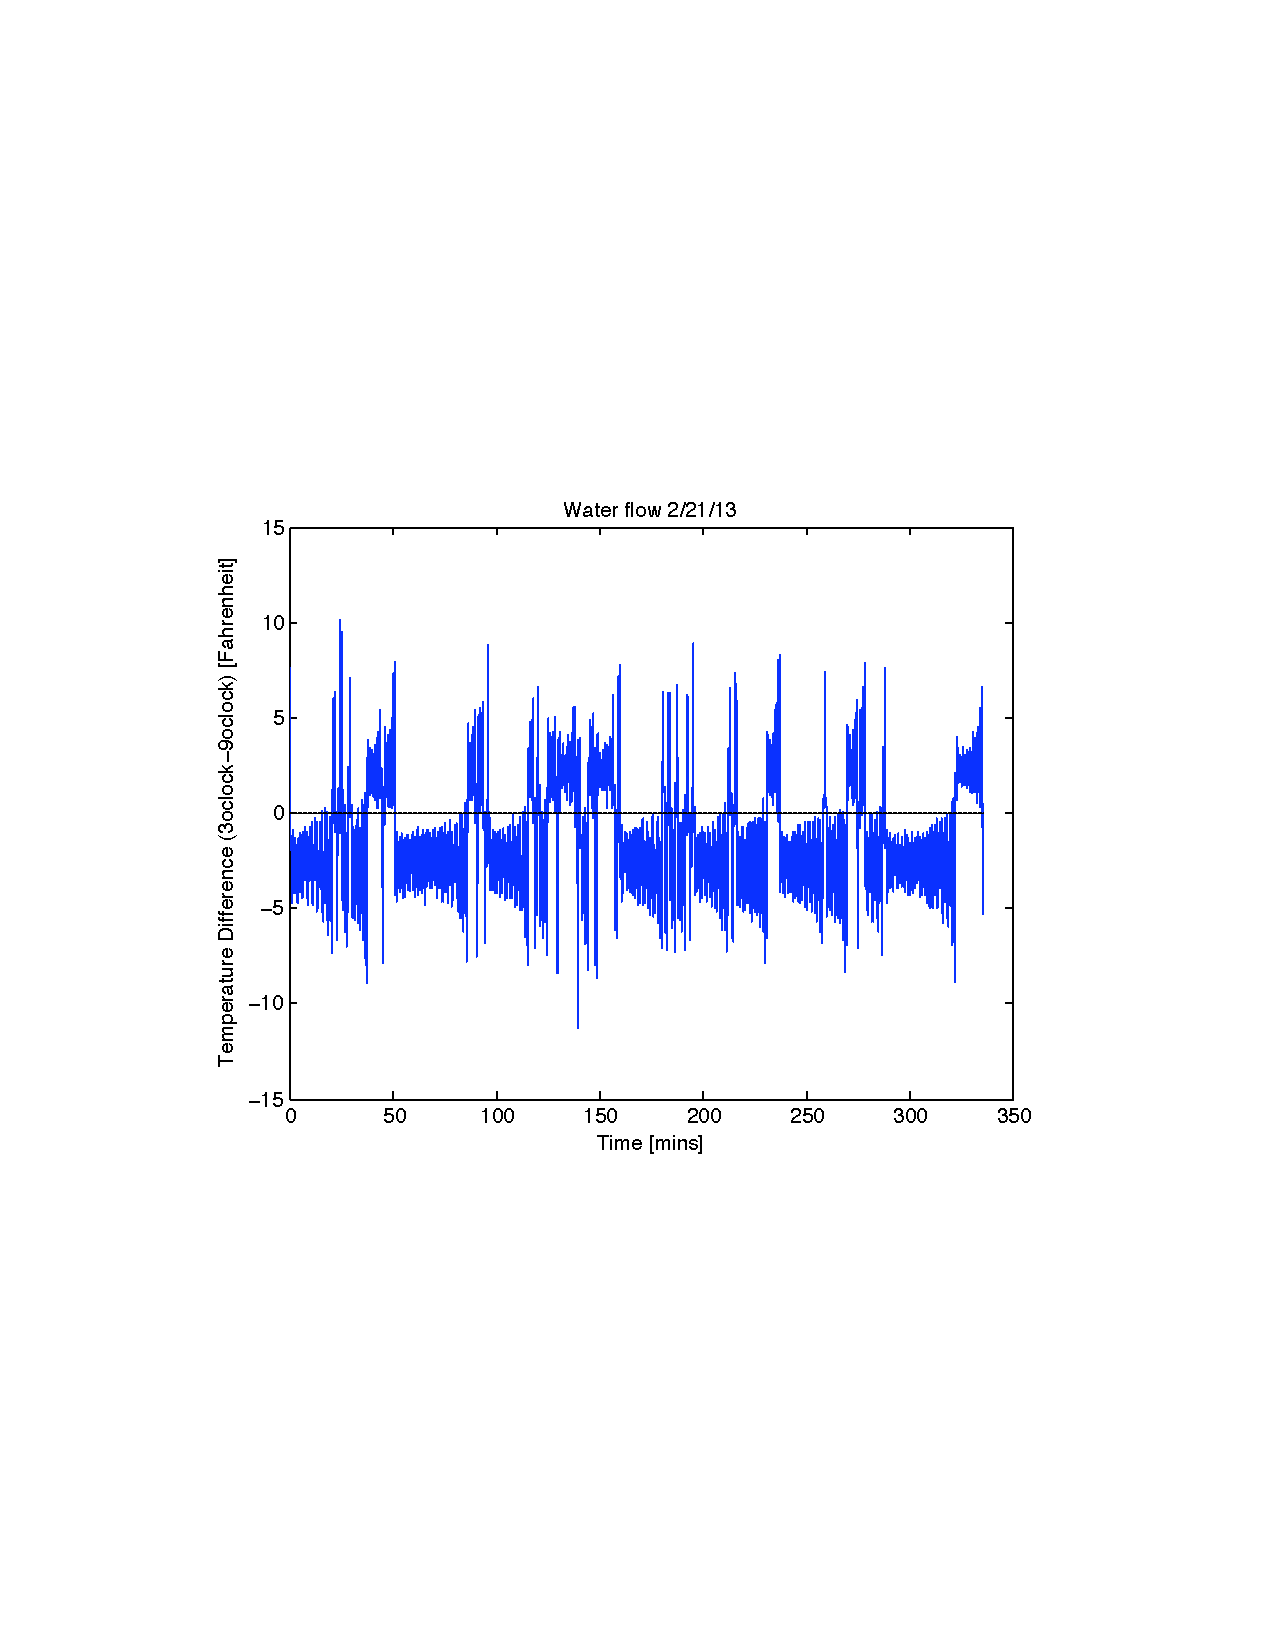
\includegraphics[width=0.45\textwidth]{figures/221TimeSeries.pdf}
  \includegraphics[width=0.5\textwidth]{/Users/andyreagan/work/2013/05-data-assimilation/thermosyphon/2015-09-30-12-26-221-timeseries.pdf}
  \caption[A time series of the physical thermosyphon, from the Undergraduate Honor's Thesis of Darcy Glenn {\protect \cite{glenn2013}}]{
    %% \the\textwidth %% 510.0pt
    A time series of the physical thermosyphon, from the Undergraduate Honor's Thesis of Darcy Glenn {\protect \cite{glenn2013}}.
    The temperature difference (plotted) is taken as the difference between temperature sensors in the 3 and 9 o'clock positions.
    The sign of the temperature difference indicates the flow direction, where positive values are clockwise flow.
  }
  \label{fig:thermosyphon-physical-timeseries}
\end{figure}

%% \begin{figure}[h!]
%%   \centering
%%   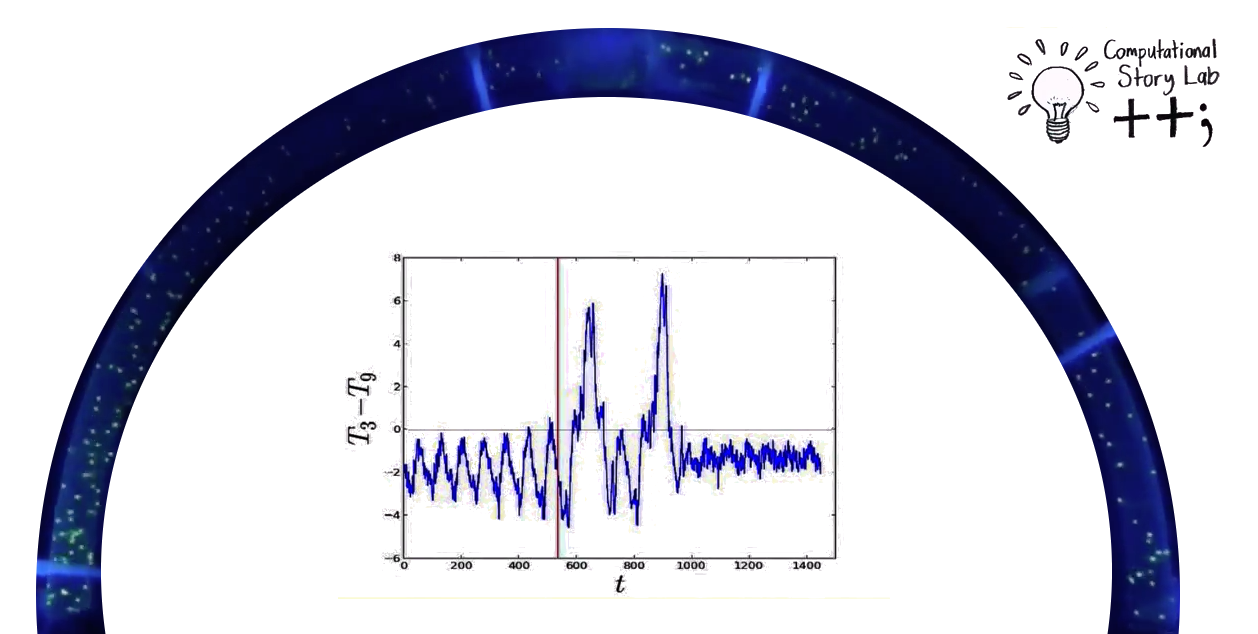
\includegraphics[width=0.45\textwidth]{figures/convectionLoopYoutubeScreenShot3.png}
%%   \caption[The Thermal Convection Loop experiment]
%%   {
%%     The Thermal Convection Loop experiment, inlaid with a time series of the temperature difference $\Delta T_{3-9}$ whose sign indicates the flow direction.
%%     Fluorescent balls are lit by a black-light and move with the flow.
%%     As the time series indicates, the flow changes direction aperiodically, giving rise to the chaotic behavior that we model.
%%     A video of the loop, from which this is a snapshot, can be viewed at \url{http://www.youtube.com/watch?feature=player_embedded&v=Vbni-7veJ-c}.
%%           }
%%   \label{fig:chrisLoop}
%% \end{figure}

Operated by Dave Hammond, UVM's Scientific Electronics Technician, the experimental thermosyphons access the chaotic regime of state space found in the principled governing equations.
We quote the detailed setup from Darcy Glenn's undergraduate thesis \cite{glenn2013} and provide Figure \ref{fig:thermosyphon-schematic} for details of the experiment:
\begin{quote}
The [thermosyphon] is a bent semi-flexible plastic tube with a 10-foot heating rope wrapped around the bottom half of the upright circle.
The tubing used is light-transmitting clear THV from McMaster-Carr, with an inner diameter of 7/8 inch, a wall thickness of 1/16 inch, and a maximum operating temperature of 200F.
The outer diameter of the circular thermosyphon is 32.25 inches.
Together, the tubing inner diameter and outer diameter of the thermosyphon produce a ratio of approximately 1:36.
There are 1 inch 'windows' when the heating cable is coiled in a helix pattern around the outside of the tube, so the heating is not exactly uniform.
The bottom half is then insulated using aluminum foil, which allowed fluid in the bottom half to reach 176F.
A forcing of 57 V, or 105 Watts, is required for the heating cable so that chaotic motion is observed.
Temperature is measured at the 3 o'clock and 9 o'clock positions using unsheathed copper thermocouples from Omega.
\end{quote}
We comfirm that the experiment accesses the chaotic regime of state space using a time series of the temperature difference as measured at the 3 o'clock and 9 o'clock positions in Figure \ref{fig:thermosyphon-physical-timeseries}.
We first test our ability to predict this experimental thermosyphon using synthetic data.
%% Synthetic data tests are the first step, since the data being predicted is generated by the predictive model.
%% We consider the potential of up to 32 synthetic temperature sensors in the loop, and velocity reconstruction from particle tracking, to gain insight into which observations will make prediction possible.

%% \subsection{Computational Setup}
We consider the incompressible Navier-Stokes equations with the Boussinesq approximation to model the flow of water inside a thermal convection loop.
For brevity, we omit the equations themselves, and include them in the Appendix.
The solver in OpenFOAM that we use, with some modification, is \verb|buoyantBoussinesqPimpleFoam|.
Solving is accomplished by the Pressure-Implicit Split Operator (PISO) algorithm \cite{issa1986solution}.
We find that modification of the code is necessary for laminar operation.

We create both 2-dimensional and 3-dimensional meshes using OpenFOAM's native meshing utility \verb|blockMesh| shown in Figures \ref{fig:CFDmesh1} and \ref{fig:CFDmesh1}.
After creating a mesh, we refine the mesh near the walls to capture boundary layer phenomena and renumber the mesh for solving speed.
We use the \verb|refineWallMesh| utility to refine the mesh near walls, and the \verb|renumberMesh| utility to renumber the mesh.
%% which implements the Cuthill-McKee algorithm to minimize the adjacency matrix bandwidth, defined as the maximum distance from diagonal of nonzero entry.
The resulting 2D mesh contains 40,000 points (40 across the diameter and 1000 around).

\begin{figure}[t]
  \centering
  \includegraphics[width=0.45\textwidth]{/Users/andyreagan/work/2013/05-data-assimilation/OpenFOAM/figures/heating_zoom_mesh4.png}
  \caption[A snapshot of the mesh used for CFD simulations]{
  A snapshot of the mesh used for CFD simulations.
  Shown is an initial stage of heating for a fixed value boundary condition, 2D, laminar simulation with a mesh of 40000 cells including wall refinement with walls heated at 340K on the bottom half and cooled to 290K on the top half.
  }
  \label{fig:CFDmesh1}
\end{figure}

\begin{figure}[t]
  \centering
  \includegraphics[width=0.45\textwidth]{/Users/andyreagan/work/2013/05-data-assimilation/OpenFOAM/figures/3D-mesh2.png}
  \caption[The 3D mesh viewed as a wire-frame from within]{
  The 3D mesh viewed as a wire-frame from within.
  Here there are 900 cells in each slice (not shown), for a total mesh size of 81,000 cells.
  Simulations using this computational mesh are prohibitively expensive for use in a real time ensemble forecasting system, but are possible offline.
  }
  \label{fig:CFDmesh2}
\end{figure}

Available boundary conditions (BCs) we find to be stable in OpenFOAM's solver are constant gradient, fixed value conditions, and turbulent heat flux.
Simulations with a fixed flux BC is implemented through the \verb|externalWallHeatFluxTemperature| library are unstable and resulted in physically unrealistic results.
Constant gradient simulations are stable, but the behavior is empirically different from our physical system.
While it is possible that a fixed value BC is acceptable due to the thermal diffusivity and thickness of the walls of the experimental setup, we find that this is also inadequate.
We employ the third-party library \verb|groovyBC| to use a gradient condition that computes a flux using a fixed external temperature and fixed wall heat transfer coefficient.

With the mesh, BCs, and solver chosen, we now simulate the flow.
From the data of $T,\phi,u,v,w$ and $p$ that are saved at each timestep, we extract the mass flow rate and average temperature at the $12,3,6$ and $9$ o'clock positions on the loop.
Since $\phi$ is saved as a face-value flux, we compute the mass flow rate over the cells $i$ of top (12 o'clock) slice as
\begin{equation} \sum _i\phi_{f(i)} \cdot v_i \cdot \rho_i\end{equation}
where $f(i)$ corresponds the face perpendicular to the loop angle at cell $i$ and $\rho$ is reconstructed from the Boussinesq approximation $\rho = \rhoref (1-\beta(T-T_\text{ref}))$.

\section{Methods}

\subsection{Data Assimilation}

We perform tests of the data assimilation algorithms described here with the Lorenz '63 system, which is analogous to the above equations with Lorenz's $\beta = 1$, and $K = 0$.
The canonical choices of $\sigma = 10, \beta = 8/3$ and $\rho = 28$ produce the well known butterfly attractor, and we use these values for all examples here.
From these tests, we will find the optimal data assimilation parameters (inflation factors) for predicting time series with this system.
Having done so, we then focus our efforts on making prediction using computational fluid dynamics models.

We first implement the 3D-Var filter.
Simply put, 3D-Var is the variational (cost-function) approach to finding the analysis.
It has been shown that 3D-var solves the same statistical problem as optimal interpolation (OI) \cite{lorenc1986analysis}.
The usefulness of the variational approach comes from the computational efficiency, when solved with an iterative method.
Specifically, the multivariate 3D-Var amounts to finding the $\mbx _a$ that minimizes the cost function
\begin{equation} J(\mbx) = (\mbx - \mbx_b) ^T \mbB ^{-1} (\mbx - \mbx_b) + (\mby_o + H(\mbx))^T\mbR (\mby_o - H(\mbx)) .\end{equation}

Next, we implement the ``gold-standard'' Extended Kalman Filter (EKF).
The tangent linear model (TLM) is precisely the model (written as a matrix) that transforms a perturbation at time $t$ to a perturbation at time $t+\Delta t$, analytically equivalent to the Jacobian of the model.
Using the notation of Kalnay \cite{kalnay2003}, this amounts to making a forecast with the nonlinear model $M$, and updating the error covariance matrix $\mbP$ with the TLM $L$, and adjoint model $L^T$:

\begin{align*} \mbx^f (t_i) &= M _{i-1} [\mbx ^a (t_{i-1} ) ],\\
\mbP^f (t_i ) &= L_{i-1} \mbP^a (t_{i-1} ) L^T _{i-1} + \mathbf{Q} (t_{i-1} ) \end{align*}

where $\mathbf{Q}$ is the noise covariance matrix (model error).
In the experiments with Lorenz '63 presented in this section, $\mathbf{Q} = 0$ since our model is perfect.
In numerical weather prediction, $\mathbf{Q}$ must be approximated, e.g., using statistical moments on the analysis increments \cite{danforth2007estimating,li2009accounting}.

The analysis step is then written as (for $H$ the observation operator):
\begin{align} \mbx^a (t_i ) &= \mbx^f (t_i) + \mbK_i \mbd_i,\\
\mbP^a (t_i) &= (\mathbf{I} - \mbK_i \mbH_i )\mbP^f (t_i) \end{align}
where
\[ \mbd_i = \mby_i^o - \mbH[x^f (t_i) ] \]
is the innovation. We compute the Kalman gain matrix to minimize the analysis error covariance $P^a _i$ as
\[ \mbK_i = \mbP^f (t_i) \mbH_i ^T [ \mbR_i + \mbH_i \mbP^f (t_i) \mbH^T ] ^{-1} \]
where $\mbR_i$ is the observation error covariance.
Since we are making observations of the truth with random normal errors of standard deviation $\mbe$, the observational error covariance matrix $\mbR$ is a diagonal matrix with $\epsilon$ along the diagonal.
The most difficult (and most computationally expensive) part of the EKF is deriving and integrating the TLM.
For this reason, the EKF is not used operationally, and later we will turn to statistical approximations of the EKF using ensembles of model forecasts.
With our CFD model we have no such TLM, and we provide more detail on the TLM approachas applicable to the Lorenz '63 system in Appendix C.

The computational cost of the EKF is mitigated through the approximation of the error covariance matrix $\mbP_f$ from the model itself, without the use of a TLM.
One such approach is the use of a forecast ensemble, where a collection of models (ensemble members) are used to statistically sample model error propagation.
With ensemble members spanning the model analysis error space, the forecasts of these ensemble members are then used to estimate the model forecast error covariance.

The only difference between this approach and the EKF, in general, is that the forecast error covariance $\mbP^f$ is computed from the ensemble members, without the need for a tangent linear model:
\[ \mbP^f \approx \frac{1}{K-2} \sum _{k\neq l} \left ( \mbx_k ^f - \overline{\mbx} ^f _l \right ) \left (\mbx_k ^f - \overline{\mbx} ^f _l \right ) ^T .\]

The ETKF introduced by Bishop is one type of square root filter, and we present it here to provide background for the formulation of the LETKF \cite{bishop2001adaptive}.
For a square root filter in general, we begin by writing the covariance matrices as the product of their matrix square roots.
Because $\mbP_a$ and $\mbP_f$ are symmetric positive-definite (by definition), we can write
\begin{equation} \mbP_a = \mbZ_a \mbZ_a^T ~~,~~~ \mbP_f = \mbZ_f \mbZ_f^T \end{equation}

\begin{figure}[t]
  \centering
  %% 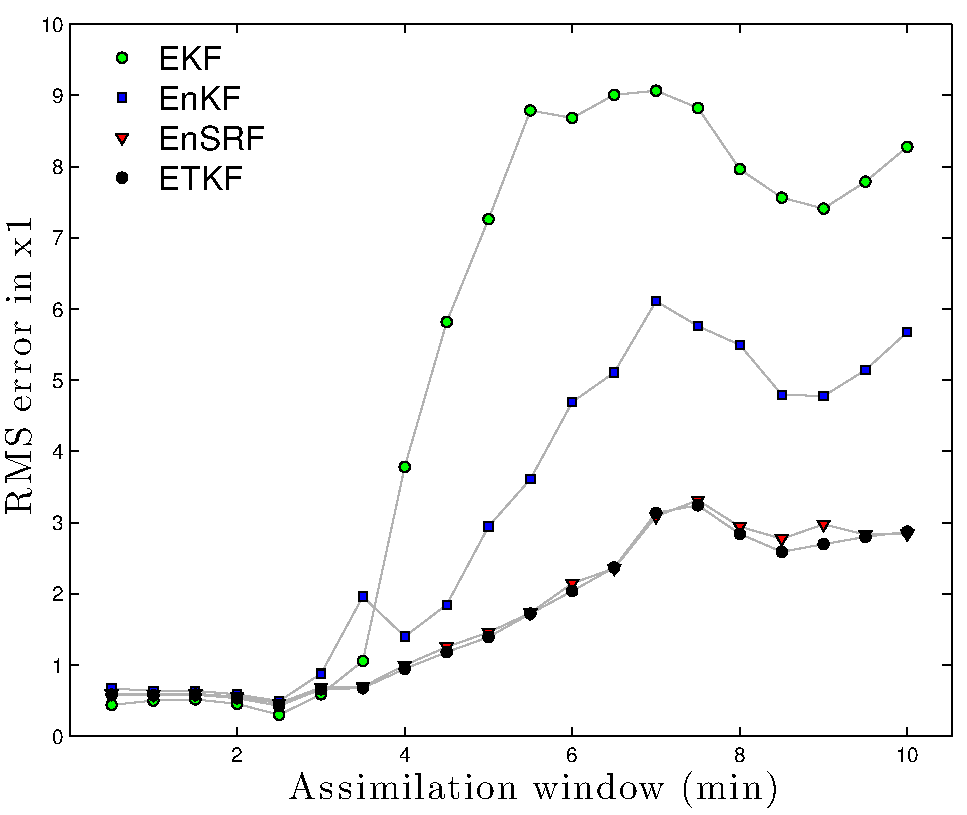
\includegraphics[width=0.45\textwidth]{figures/window_experiment_plot002.pdf}
  \includegraphics[width=0.50\textwidth]{/Users/andyreagan/work/2013/05-data-assimilation/src/experiments/windowExperiment/2015-09-30-14-17-window-experiment.pdf}
  \caption[The RMS error is reported for our EKF and EnKF filters]{
    The RMS error (not scaled by climatology) for our EKF and EnKF filters, measured as the difference between forecast and truth at the end of an assimiliation window for the latter 2500 assimiliation windows in a 3000 assimilation window Lorenz '63 run.
    Error is measured in the only observed variable, $x_1$.
    Increasing the assimilation window led to an decrease in predictive skill, as expected.
  }
  \label{fig:window_test}
\end{figure}

\begin{figure}[t]
  \centering
  %% 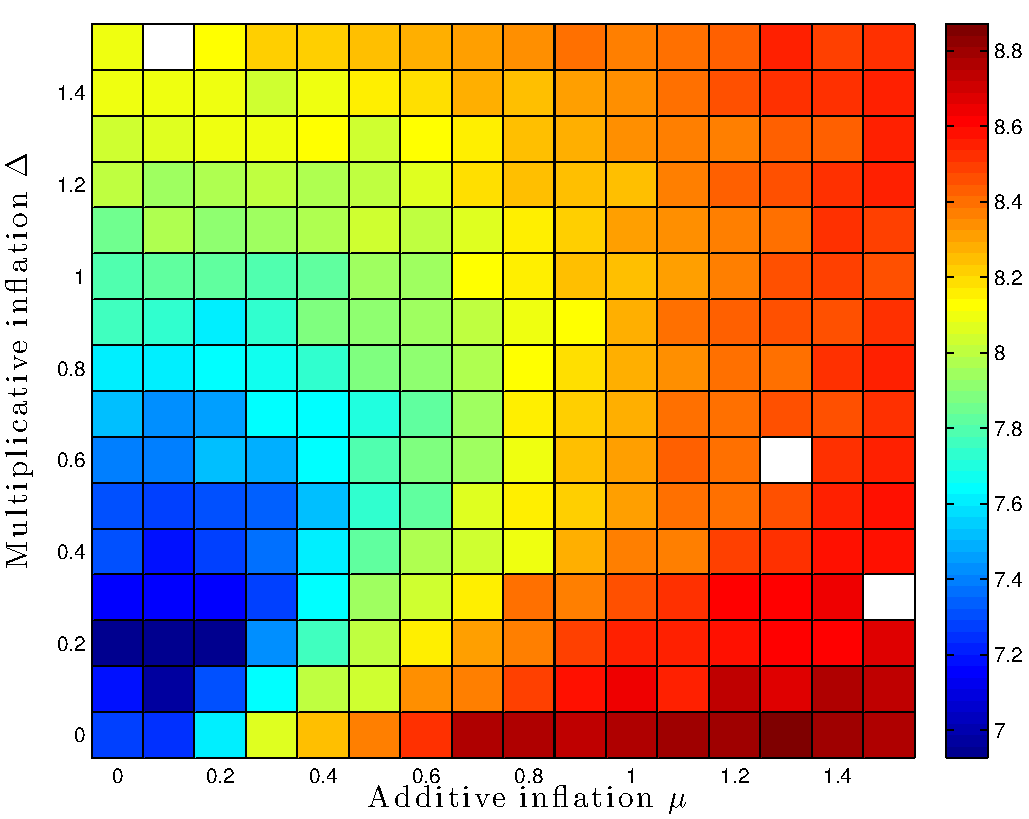
\includegraphics[width=0.45\textwidth]{figures/ETKF_390s_infl_error.pdf}
  \includegraphics[width=0.48\textwidth]{/Users/andyreagan/work/2013/05-data-assimilation/src/experiments/covInflTest/2015-09-30-15-35-ETKF-390s.pdf}
  \caption[The RMS error averaged over 100 model runs of length 1000 windows is reported for the ETKF for varying additive and multiplicative inflation factors]{
    The RMS error averaged over 100 model runs of length 1000 windows is reported for the ETKF for varying additive and multiplicative inflation factors $\Delta$ and $\mu$.
    Each of the 100 model runs starts with a random IC, and the analysis forecast starts randomly.
    The window length here is 390 seconds.
    The filter performance RMS is computed as the RMS value of the difference between forecast and truth at the assimilation window for the latter 500 windows, allowing a spin-up of 500 windows.
  }
  \label{fig:ETKF_cov_tuning_390s}
\end{figure}

where $\mbZ_a$ and $\mbZ_f$ are the matrix square roots of $\mbP_a$ and $\mbP_f$.
We are not concerned that this decomposition is not unique, and note that $\mbZ$ must have the same rank as $\mbP$ which will prove computationally advantageous.
The power of the SRF is now seen as we represent the columns of the matrix $\mbZ_f$ as the difference from the ensemble members from the ensemble mean, to avoid forming the full forecast covariance matrix $\mbP_f$.
The ensemble members are updated by applying the model $M$ to the states $\mbZ_f$ such that an update is performed by
\begin{equation} \mbZ_f = M \mbZ_a .\end{equation}
To summarize, the steps for the ETKF are to (1) form $\mbZ_f^T\mbH^T\mbR^{-1}\mbH\mbZ_f$, assuming that computing $\mathbf{R}^{-1}$ is easy, and (2) compute its eigenvalue decomposition, and apply it to $\mbZ_f$.

The LEKF implements a strategy that becomes important for large simulations: localization.
Namely, the analysis is computed for each grid-point using only local observations, without the need to build matrices that represent the entire analysis space.
Localization removes long-distance correlations from $\mathbf{B}$ and allows greater flexibility in the global analysis by allowing different linear combinations of ensemble members at different spatial locations \cite{kalnay20074}.
The general formulation of the LEKF by Ott goes as follows, quoting directly from \cite{ott2004local}:
\begin{enumerate}
\item Globally advance each ensemble member to the next analysis timestep. Steps 2--5 are performed for each grid point.
\item Create local vectors from each ensemble member.
\item Project that point's local vectors from each ensemble member into a low dimensional subspace as represented by perturbations from the mean.
\item Perform the data assimilation step to obtain a local analysis mean and covariance.
\item Generate local analysis ensemble of states.
\item Form a new global analysis ensemble from all of the local analyses.
\item Wash, rinse, and repeat.
\end{enumerate}

Proposed by Hunt in 2007 with the stated objective of computational efficiency, the LETKF is named from its most similar algorithms from which it draws \cite{hunt2007efficient}.
With the formulation of the LEKF and the ETKF given, the LETKF can be  described as a synthesis of the advantages of both of these approaches.
The LETKF is the method sufficiently efficient for implementation on the full OpenFOAM CFD model of 240,000 model variables, and so we present it in more detail and follow the notation of Hunt \etal (2007). 
As in the LEKF, we explicitly perform the analysis for each grid point of the model.
The choice of observations to use for each grid point can be selected a priori, and tuned adaptively.
Starting with a collection of background forecast vectors $\{ \mbx_{b(i)}:\,i=1,\ldots,k \}$, we perform steps 1 and 2 in a global variable space, then steps 3--8 for each grid point:
\begin{enumerate}
\item Apply $H$ to $\mbx_{b(i)}$ to form $\mby_{b(i)}$, average the $\mby_b$ for $\overline{\mby_b}$, and form $\mbY b$.
\item Similarly form $\mbX_b$. Now for each grid point:
\item Form the local vectors.
\item Compute $\mathbf{C}=(\mbY_b)^T\mbR^{-1}$ (perhaps by solving $\mbR \mathbf{C}^T = \mbY_b$.
\item Compute $\tilde{\mbP}_a = \left( (k-1)\mathbf{I} / \rho + \mathbf{C} \mbY _b \right ) ^{-1}$ where $\rho > 1$ is a tun-able covariance inflation factor.
\item Compute $\mbW_a = \left ( (k-1) \tilde{\mbP} _a \right ) ^{1/2}$.
\item Compute $\overline{\mbw} _a  = \tilde{\mbP}_a \mathbf{C} \left ( \mby_o - \overline{\mby} _b \right )$ and add it to the column of $\mbW_a$.
\item Multiply $\mbX_b$ by each $\mbw_{a(i)}$ and add $\tilde{\mbx}_b$ to get $\left\{ \mbx_{a(i)}:\,i=1,\ldots,k\right \}$ to complete each grid point.
\item Combine all of the local analysis into the global analysis.
\end{enumerate}
We implement the LETKF on our mesh using the full 40 cells across with zone sizes of center 10, and sides 15, resulting in 1600 local variables for 100 zones.
In parallel, these 100 local computations can all be carried out simultaneously over an arbitrary number of processors.

\subsection{Adaptive covariance localization}

Using the ``square'' sections of the loop to localize, we shift the zone to the left or right to follow the dominate flow direction at the center of that local window.
In Figure \ref{fig:covariance-localization-schematic} a schematic of localization using square, circular, and adpative location shows a situation in which adaptive localization will potentially capture more relevant information for finding the analysis state of any given cell.
As we note in the caption of Figure \ref{fig:covariance-localization-schematic}, while we are motivated by localization around flow structures like Panel C, we simply shift the covariance in Panel A so that our method is most general and computationally efficient.

Denote the velocity vector of cells on a perpendicular slice of the loop at $\vec{U}$, the tangent vector to the slice $\vec{U}$ by $\vec{T}$, the zone width as $z_{\text{max}}$ and then the localization shift $\alpha_{\text{local}}$ for that slice of the loop is taken to be
\begin{equation} \alpha_{\text{local}} = \text{floor} \left( (\vec{U} \cdot \vec{T})/\max (U) \times z_{\text{max}} \right) . \end{equation}

\subsection{Dynamic mode decomposition}

We employ the ``standard'' algorithm of Tu to compute the Dynamic Mode Decomposition \cite{tu2013dynamic}.
Tu's ``standard'' algorithm is as follows with $X$ and $Y$ taken as the first and last $N-1$ columns of the snapshot matrix $D$:
\begin{align*} X &= U\Sigma V \tag*{(Take SVD of $X$.)}\\
  \tilde{A} &= U^T Y V \Sigma ^{-1} \tag*{(Build the $A$ matrix.)}\\
  \tilde{A}w &= \lambda w \tag*{(Compute eigenvectors and values.)}\\
  \hat{\theta}w &= U w \tag*{(Compute corresponding modes.)}\end{align*}

Given a system state $U^*$ we project this state onto the DMD basis by taking the real part of $U^*\cdot w = \Phi$ and use the psuedoinverse to compute the projection $(\Phi^T \cdot \Phi)^{-1} \cdot \Phi ^T \cdot U^*$.

\section{Results}

\subsection{Data assimilation}

We confirm the performance of the DA methods described above by testing each (on the Lorenz '63 system) for increasingly long times between observations, by increasing the DA window length in Figure \ref{fig:window_test}.
As the time between observations increases, the nonlinearity of the Lorenz '63 system results in the failure of the EKF and difficultly for the EnKF with small ensemble size.
The ETKF and EnSRF perform the best of the methods tested and we chose the ETKF for future use with the CFD model.

The results in Figure \ref{fig:window_test} rely on tuned covariance inflation, both additive and multiplicative, pre-computed for each window and DA technique.
We choose optimal additive inflation $\mu$ and multiplicative inflation $\Delta$ by selecting for the lowest error in an exhaustive search through a maximum factors of $1.5$ in each, an example is shown in Figure \ref{fig:ETKF_cov_tuning_390s}.
We use these optimal data assimilation parameters (inflation factors) for the remainder of this work.

\subsection{Limited observations \& adaptive covariance}

An initial test of prediction skill with limited observations in a twin model experiment showed that we needed 1000 spatial measurements of the temperature to predict flow reversals within 1 assimilation window.
In an attempt to decrease the required observations to a experimentally realizable number, we implement a simple, adaptively localized covariance for data assimilation.
Since we first saw a modest improvement in the prediction skill with full temperature observations, we hope that this improvement increases and is sufficient to get down to needing as few as 32 observations to predict reversals 1 assimilation window (of length 10 seconds) into the future.

In Figure \ref{fig:sliding_spag} we see that over an assimilation of 200 seconds, the ensemble converges on the hidden, true state.
To test the performace of flow reversal prediction, we take the average of the ensemble flow direction (the average of each value of $\phi$) as the predicted flow direction, and count how often we predict reversals both when they do and do not occur.
Varying both the number of model variables and the strength of convariance shifting in Figure \ref{fig:sliding_results}, we find that covariance shifting improves flow reversal prediction skill even when overservations are decreased.
With full observations (spacing of 1), we obtain a the best predictions with a covariance shift of 2.
For 1/2 and 1/5 observations [a spacing of 2 (5) to obvserve every other (fifth) variable], we again have the best predictions with a shift of 2.
And for a spacing of 10, observing every 10th variable, we achieve greater prediction skill with a covariance shift of 10.

Computing the average flow direction inside a localized covariance zone is straighforward, and computationally easy since the velocity is immediately available, making incorporation of this scheme into any data assimilation method easy.
Since observations are also sparse in large weather models, we expect that using an adaptive local covariance scheme could lead to improved prediction skill.

\begin{figure}[t]
  \centering
  %% 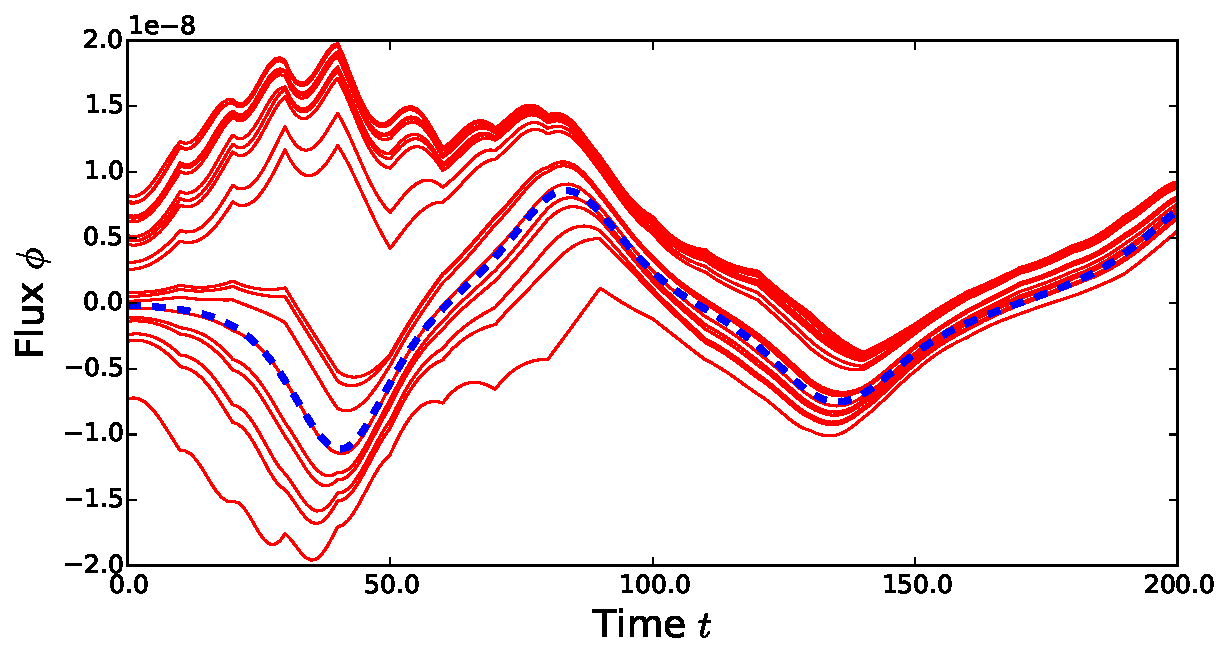
\includegraphics[width=0.45\textwidth]{../figures/loop-spaghetti-slide-004-full.pdf}
  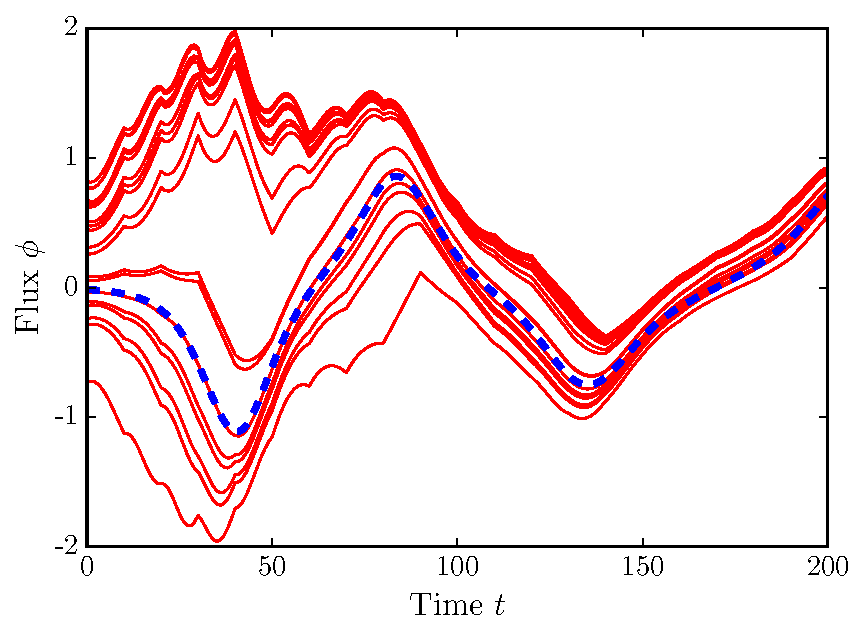
\includegraphics[width=0.48\textwidth]{../figures/2015-09-30-15-48-loop-spaghetti.pdf}
  \caption[]{
    Convergence of 20 ensembles using sliding windows, starting from initially random states.
    Here, as in most of the experiments, only temperature is observered and assimilated.
    Flux is computed as in Equation 4, on the left hand side of the thermosyphon, and scaled by a factor of $10^8$.
    Assimilation takes place every 10 model seconds.
  }
  \label{fig:sliding_spag}
\end{figure}

\begin{figure}[t]
  \centering
  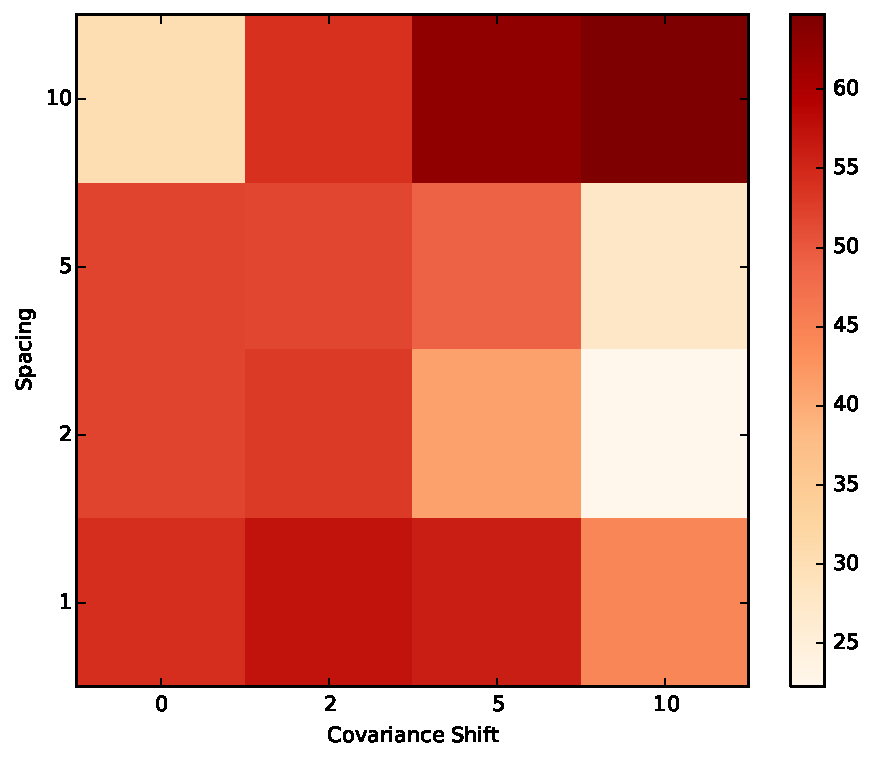
\includegraphics[width=0.45\textwidth]{../figures/2015-09-13-23-04-consuela.pdf}
  \caption[]{
    Prediction skill as fraction of reversals that we correctly predicted across different numbers of observations and sliding windows of localized covariance.
  }
  \label{fig:sliding_results}
\end{figure}

\subsection{Dynamic mode decomposition}

\begin{figure}[t]
  \centering
  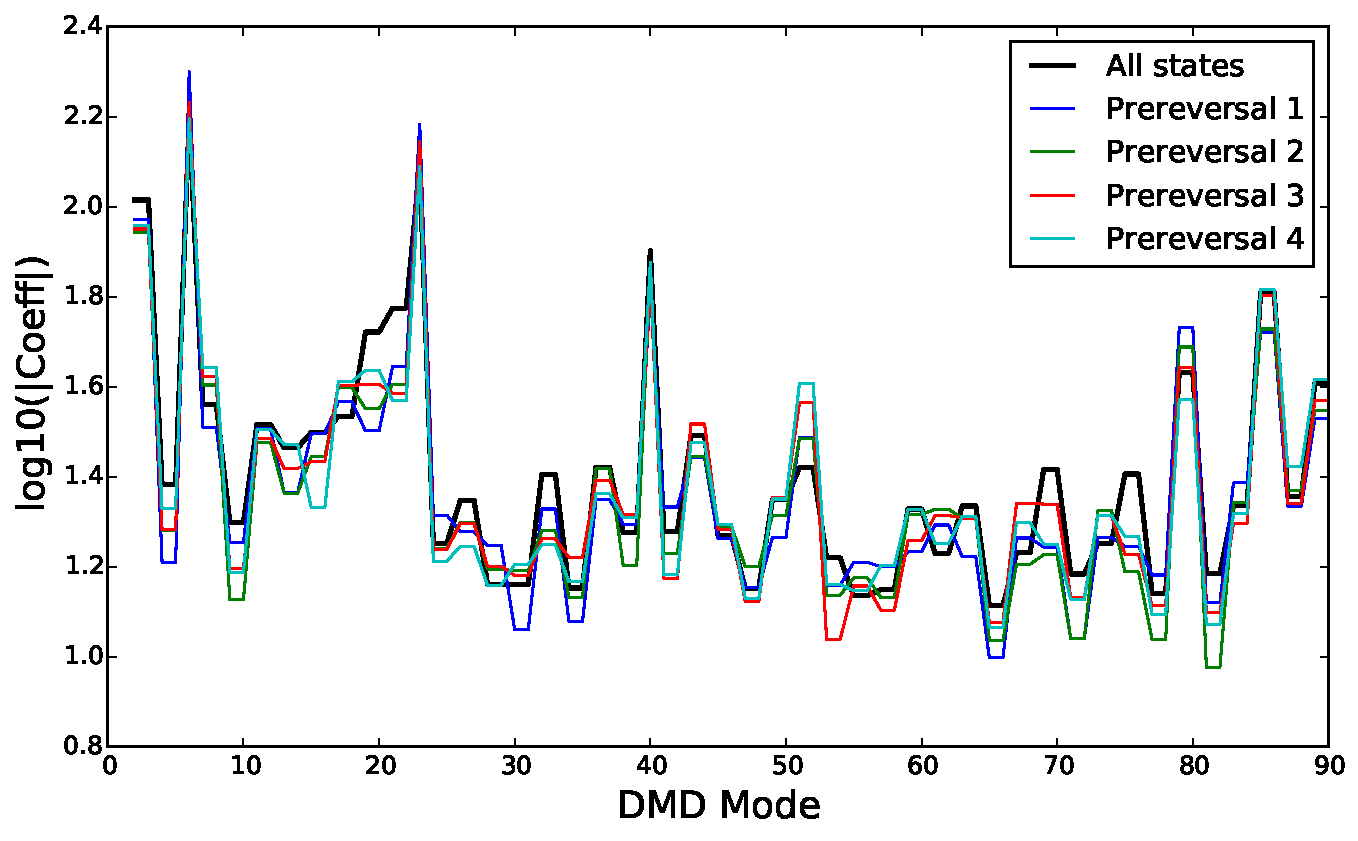
\includegraphics[width=0.45\textwidth]{../figures/DMD/DMD_modes_pre_reversals.pdf}
  \caption[]{
    The $\log_{10}$ average projection onto each DMD mode for different sets of model states.
    DMD constructed as snapshots every 10 seconds for the first 900 seconds of model time, and model states from the first 2000 seconds are all projected onto the DMD modes.
    All states average shown in black, and the average of the subset of states that occur 1 second, 3 seconds, 5 seconds, and 7 seconds before a reversal are shown in other colors.
    The symmetry of the loop generates modes that often come in pairs.
      }
  \label{fig:DMD_modes}
\end{figure}

%% \begin{figure}[t]
%%   \centering
%%   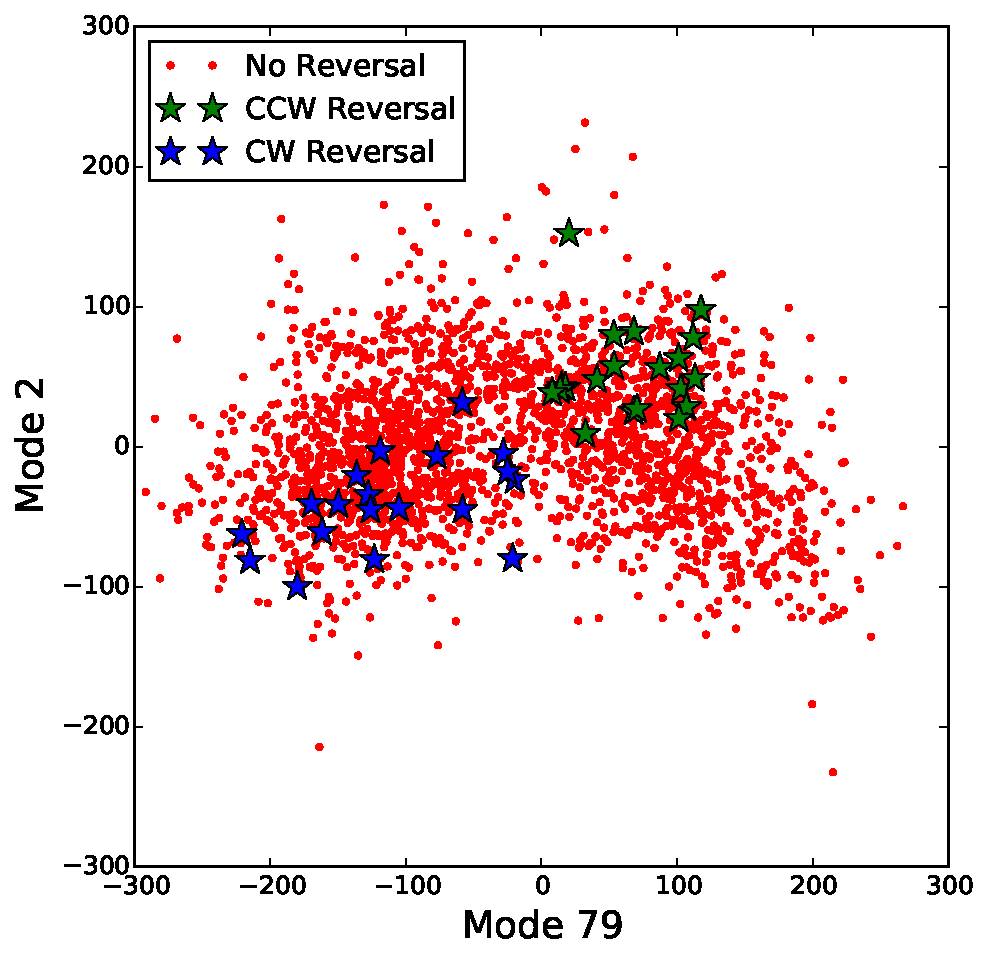
\includegraphics[width=0.45\textwidth]{../figures/DMD/DMD_mode_2_79_phaseplane-003.pdf}
%%   \caption[]{
%%     This butterfly-shaped phase plane shows the value of the projection onto modes 2 and 79 for each time in the first 2000 timesteps of our ground truth model run.
%%     In blue and green stars the states that occur directly before a flow are highlighted, and are isolated into separate quadrants of phase space.
%%     \todo{Make 3-panel, full width figure}
%%   }
%%   \label{fig:DMD_phaseplane}
%% \end{figure}

%% the stacked figures are made by pasting the png time series on top of the png loops in preview, and stretching the png time series to be from the left edge to .25 on x, then centering vertically using the dragging circles, and horizontally by eye
%% then we combine them into labeled and unlabeled versions like this:
%% ~/work/2015/08-kitchentabletools/pdftile.pl 1 3 .3 0 0 l 12 "" "" DMD-mode02-tu-Wu-stacked.png "" DMD-mode79-tu-Wu-stacked.png "" ../../figures/DMD/DMD_mode_2_79_phaseplane-003.pdf combined-phase-potrait-2-79
%% but here, first go modify pdftile to wrap the titles in a ``footnotesize''
%% ~/work/2015/08-kitchentabletools/pdftile.pl 1 3 .34 0 0 l 10 "" "A: Mode 2" DMD-mode02-tu-Wu-stacked.png "B: Mode 79" DMD-mode79-tu-Wu-stacked.png "C: Phase Plane" ../../figures/DMD/DMD_mode_2_79_phaseplane-003.pdf combined-phase-potrait-2-79-labeled

\begin{figure*}
  \centering
  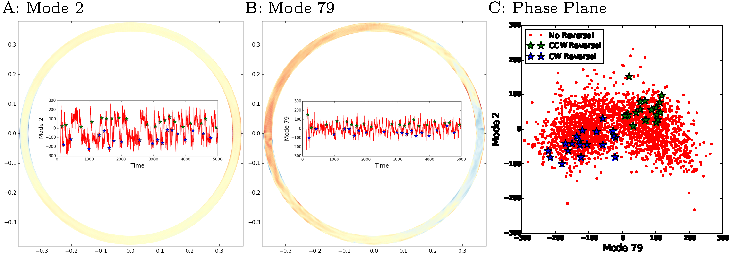
\includegraphics[width=0.98\textwidth]{figures/combined-phase-potrait-2-79-labeled.pdf}
  \caption[]{
    Panel A: The temperature profile of the thermosyphon of Mode 2, with inset of the projection of time series states onto Mode 2 (the projection coefficient).
    Panel B: Likewise, the temperature profile of the thermosyphon of Mode 79, with inset of the projection of time series states onto Mode 79 (the projection coefficient).
    Panel C: A butterfly-shaped phase plane shows the value of the projection onto modes 2 and 79 for each time in the first 2000 timesteps of our ground truth model run.
    In blue and green stars the states that occur directly before a flow are highlighted, and are isolated into separate quadrants of phase space.
  }
  \label{fig:DMD_phaseplane}
\end{figure*}

%% ~/work/2015/08-kitchentabletools/pdftile 3 1 .9 0 0 c 10 "" "" foamlab_slides002.pdf "" foamlab_slides003.pdf "" foamlab_slides004.pdf covariance-localization-schematic
%% ~/work/2015/08-kitchentabletools/pdftile.pl 3 1 .9 0 0 c 10 "" "" foamlab_slides002.pdf "" foamlab_slides003.pdf "" foamlab_slides004.pdf covariance-localization-schematic
%% open covariance-localization-schematic.pdf 
%% ~/work/2015/08-kitchentabletools/pdftile.pl 3 1 .9 0 0 c 10 "" "A: Square Covariance" foamlab_slides002.pdf "B: Circular Covariance" foamlab_slides003.pdf "C: Adaptive Covariance" foamlab_slides004.pdf covariance-localization-schematic-labeled
%% ~/work/2015/08-kitchentabletools/pdftile.pl 3 1 .9 0 0 c 12 "" "A: Square Covariance" foamlab_slides002.pdf "B: Circular Covariance" foamlab_slides003.pdf "C: Adaptive Covariance" foamlab_slides004.pdf covariance-localization-schematic-labeled-002
%% try to make it bigger, but fontsize only goes to 12
%% ~/work/2015/08-kitchentabletools/pdftile.pl 3 1 .9 0 0 c 14 "" "A: Square Covariance" foamlab_slides002.pdf "B: Circular Covariance" foamlab_slides003.pdf "C: Adaptive Covariance" foamlab_slides004.pdf covariance-localization-schematic-labeled-003
%% edit the pdftile.pl to give it a Large
%% ~/work/2015/08-kitchentabletools/pdftile.pl 3 1 .9 0 0 c 12 "" "A: Square Covariance" foamlab_slides002.pdf "B: Circular Covariance" foamlab_slides003.pdf "C: Adaptive Covariance" foamlab_slides004.pdf covariance-localization-schematic-labeled-004
%% ~/work/2015/08-kitchentabletools/pdftile-adjustlabelsize.pl 3 1 .9 0 0 c Large "" "A: Square Covariance" foamlab_slides002.pdf "B: Circular Covariance" foamlab_slides003.pdf "C: Adaptive Covariance" foamlab_slides004.pdf covariance-localization-schematic-labeled-005

\begin{figure}[t]
  \centering
  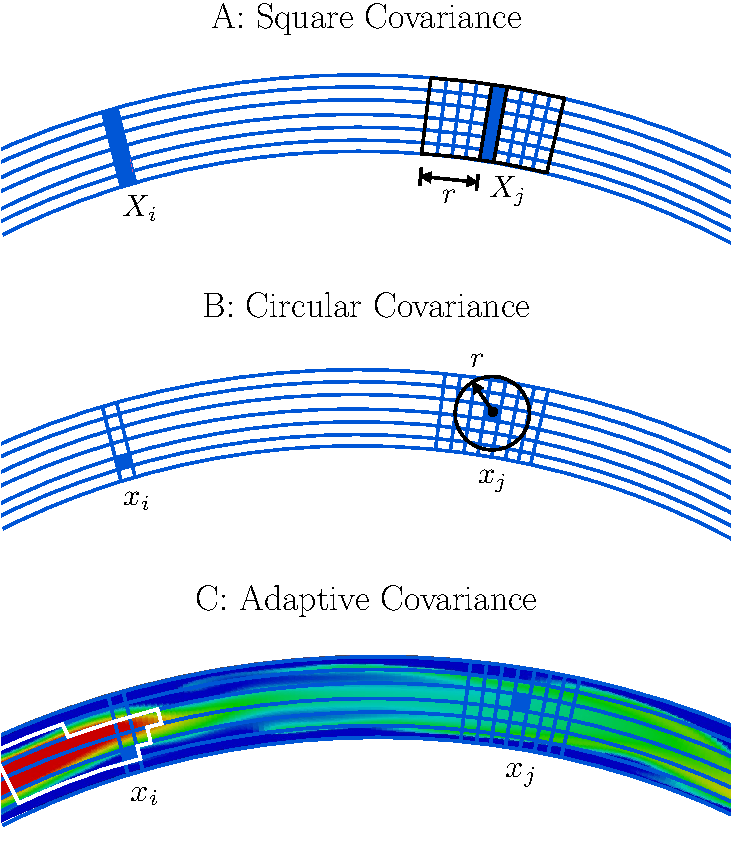
\includegraphics[width=0.45\textwidth]{figures/covariance-localization-schematic-labeled-004.pdf}
  \caption[]{
    Schematic of the adaptive covariance localization.
    In Panel A we see a zonal (square) covariance that is most similar to the covariance used for both control sliding covariance.
    Panel B shows a localized covariance using a ``local radius'', and Panel C shows an idealized, fully adaptive covariance.
    While we are motivated by localization around flow structures like Panel C, we simply shift the covariance in Panel A so that our method is most general and computationally efficient.
  }
  \label{fig:covariance-localization-schematic}
\end{figure}

To incorporate limited observations into a high-dimensional CFD simulation, we combine ideas from both CFD literature and data assimilation to make predictions.
%% We perform data assimilation in a subspace composed of the leading modes from a DMD of a series of loop snapshots.
We proceed with Tu's algorithm using snapshots every 10 seconds for the first 900 seconds of model time.
A full picture of this time series can be found Appendix C, Figure \ref{fig:DMD-timeseries}.

In this reduced space, we extract the modes that correspond to the instability leading to flow reversals.
For modes 21 and 79, we directly observe in Figure \ref{fig:DMD_modes} that the average projection from states just 1 second before reversal is the most different from the average stat projection, and the further away from the reversal, the more similiar the states become to the average.
In Figure \ref{fig:DMD_phaseplane} we see that the dominant dynamics from mode 2 plotted with those of mode 79 are able to strongly separate reversal.

\section{Concluding Remarks}

The first output of our work is a general data assimilation framework for MATLAB and Julia.
By utilizing an object-oriented (OO) design, the model and data assimilation algorithm code are separate and can be changed independently.
The principal advantage of this approach is the ease of incorporation of new models and DA techniques (code available at \url{https://github.com/andyreagan/julia-openfoam}).

We first present the results pertaining to the accuracy of forecasts for synthetic data (twin model experiments).
There are many possible experiments given the choice of assimilation window, data assimilation algorithm, localization scheme, model resolution, observational density, observed variables, and observation quality.
We focused on considering the effect of observations and observational locations on the resulting forecast skill, and we find that there is a threshold for the required number of observations to make useful predictions.
In general, we see that increasing observational density leads to improved forecast accuracy.
With too few observations, the data assimilation is unable to recover the underlying dynamics.
Using adaptively localized covariance holds promise for data assimilation with data-scarce models, to overcome the lack of data.

The ability of DMD to recover the lower dimensional dynamics is expected but with 120,000 variables is nonetheless an accomplishment.
When modeling systems for which there are unknown but useful dimension reductions, as demonstrated here, DMD can be a useful tool.

The numerical coupling of CFD to experiment by DA should be generally useful to improve the skill of CFD predictions in even data-poor experiments, which can provide better knowledge of unobservable quantities of interest in fluid flow.


